\section{Resultados}

\begin{frame}{\insertsectionhead}
    \framesubtitle{Función de Rosembrock}
    La función de Rosembrock se define en la ecuación \ref{eq:rosembrock}.

    \begin{equation}
        f(x) = \sum_{i=1}^{n-1}  100(x_{i+1}-x_{i}^2)^2 +(1-x_i)
        \label{eq:rosembrock}
    \end{equation}
\end{frame}

\begin{frame}{\insertsectionhead}
    \framesubtitle{Función Wood}
    La función de Wood se define en la ecuación \ref{eq:wood}.

    \tiny
    \begin{equation}
        f(x) = 100(x_1^2-x_2)^2+(x_1-1)^2+(x_3-1)^2+90(x_3-x_4)^2 +10.1((x_2-1)^2+(x_4-1)^2)+19.8(x_2-1)(x_4-1) \label{eq:wood}
    \end{equation}
\end{frame}

\begin{frame}{\insertsectionhead}
    \framesubtitle{Función Lambda}
    En el artículo de Yakui Huang se utiliza una función definida de la siguiente manera:

    \begin{equation*}
        f(x) = \frac{1}{2}x^TAx \qquad A=\begin{cases}
            0                           & \text{para } i\neq 0 \\
            10^{\frac{ncond}{n-1}(n-j)} & \text{para } i=j
        \end{cases}
    \end{equation*}

    donde $ncond=log \kappa$ con $\kappa = 10^3$ y $n=10$.
\end{frame}

\begin{frame}{\insertsectionhead}
    \framesubtitle{Función cuadrática}
    En el mismo artículo\cite{huang_2022_1} se propone una función cuadrática donde la matriz esta definida de la siguiente manera:

    \begin{equation*}
        A = diag\{1,\lambda\}
    \end{equation*}

    En nuestro caso tomamos $\lambda=10$.
\end{frame}

\begin{frame}{\insertsectionhead}
    \framesubtitle{Porcentaje de contribución}
    Se definió una función $\gamma$ para medir el porcentaje de las dos componentes más grandes del gradiente en cada iteración de la optimización. La función $\gamma$ tiene la siguiente forma

    \begin{equation*}
        \gamma(g_k) = \frac{|g_k^{(1)}|+|g_k^{(2)}|}{\sum\limits_i |g_k^{(i)}|}
    \end{equation*}

    Realizando el calculo de la función $\gamma$ con la función lambda en el punto inicial $x=(10,10,\dots,10)^T$ se obtuvieron los resultados mostrados en la figura \ref{fig:gamma} para los diferentes métodos.
\end{frame}

\begin{frame}
    \vspace{0.5cm}
    \begin{figure}[H]
        \begin{subfigure}{7cm}
            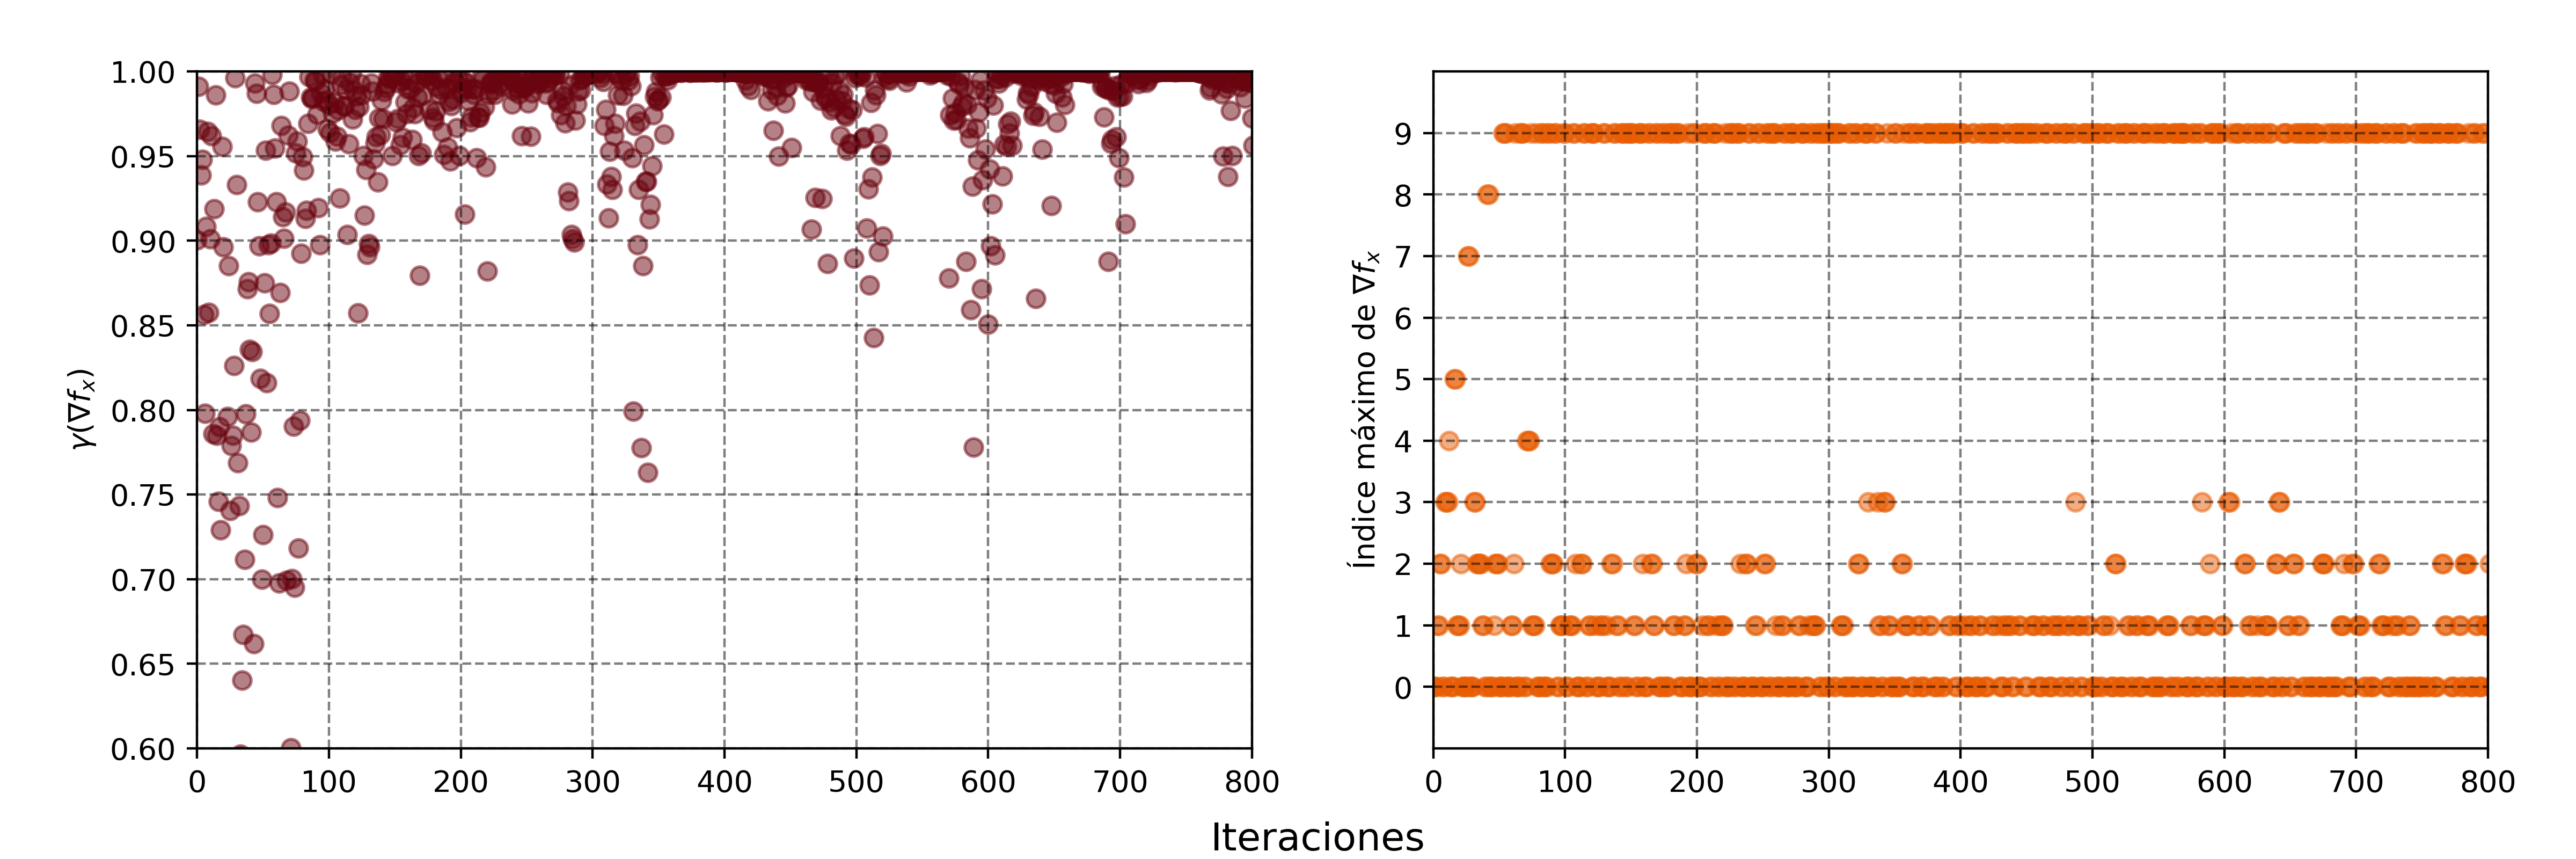
\includegraphics[width=1\textwidth]{Graphics/gamma/barzilai.png}
            \caption{Método BB.}
        \end{subfigure}
        \begin{subfigure}{7cm}
            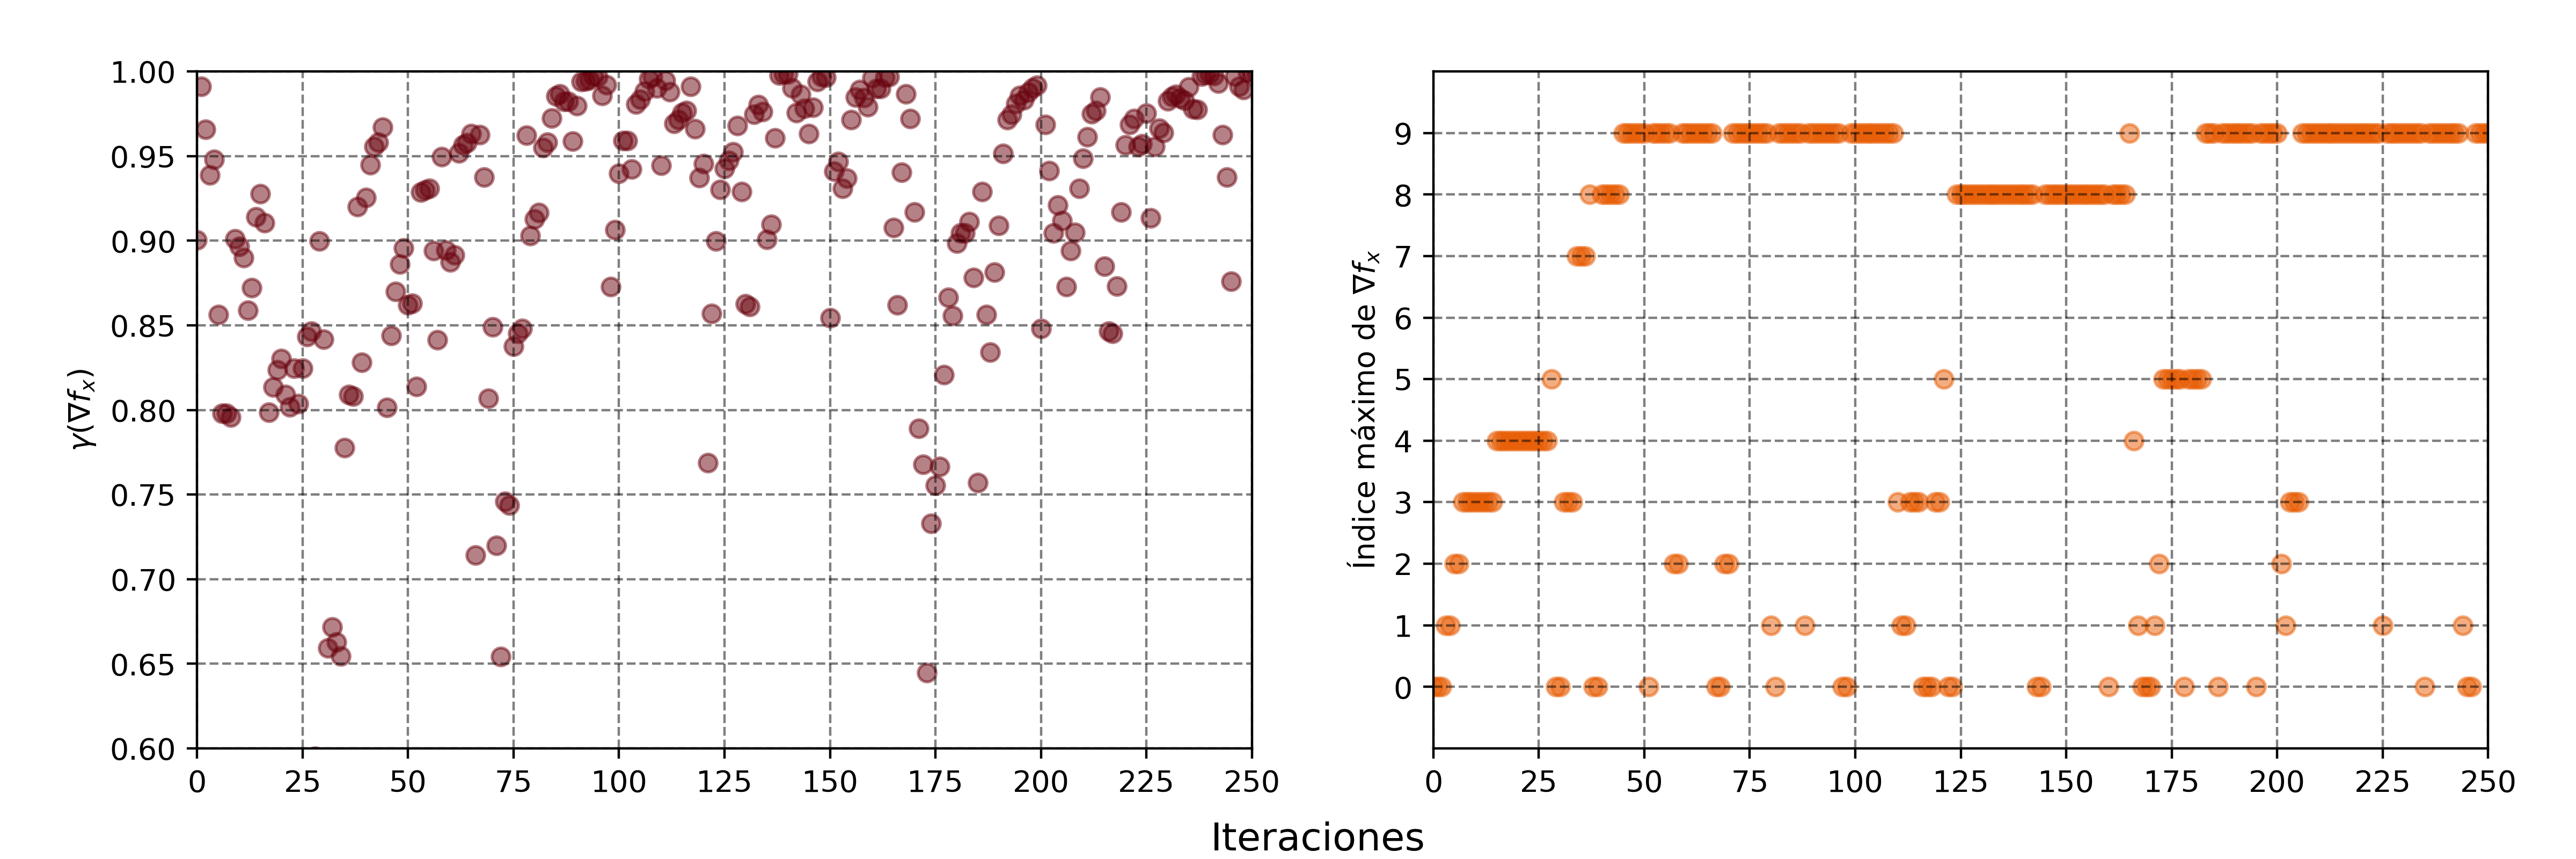
\includegraphics[width=1\textwidth]{Graphics/gamma/ANGM.png}
            \caption{Método ANGM.}
        \end{subfigure}
        \begin{subfigure}{7cm}
            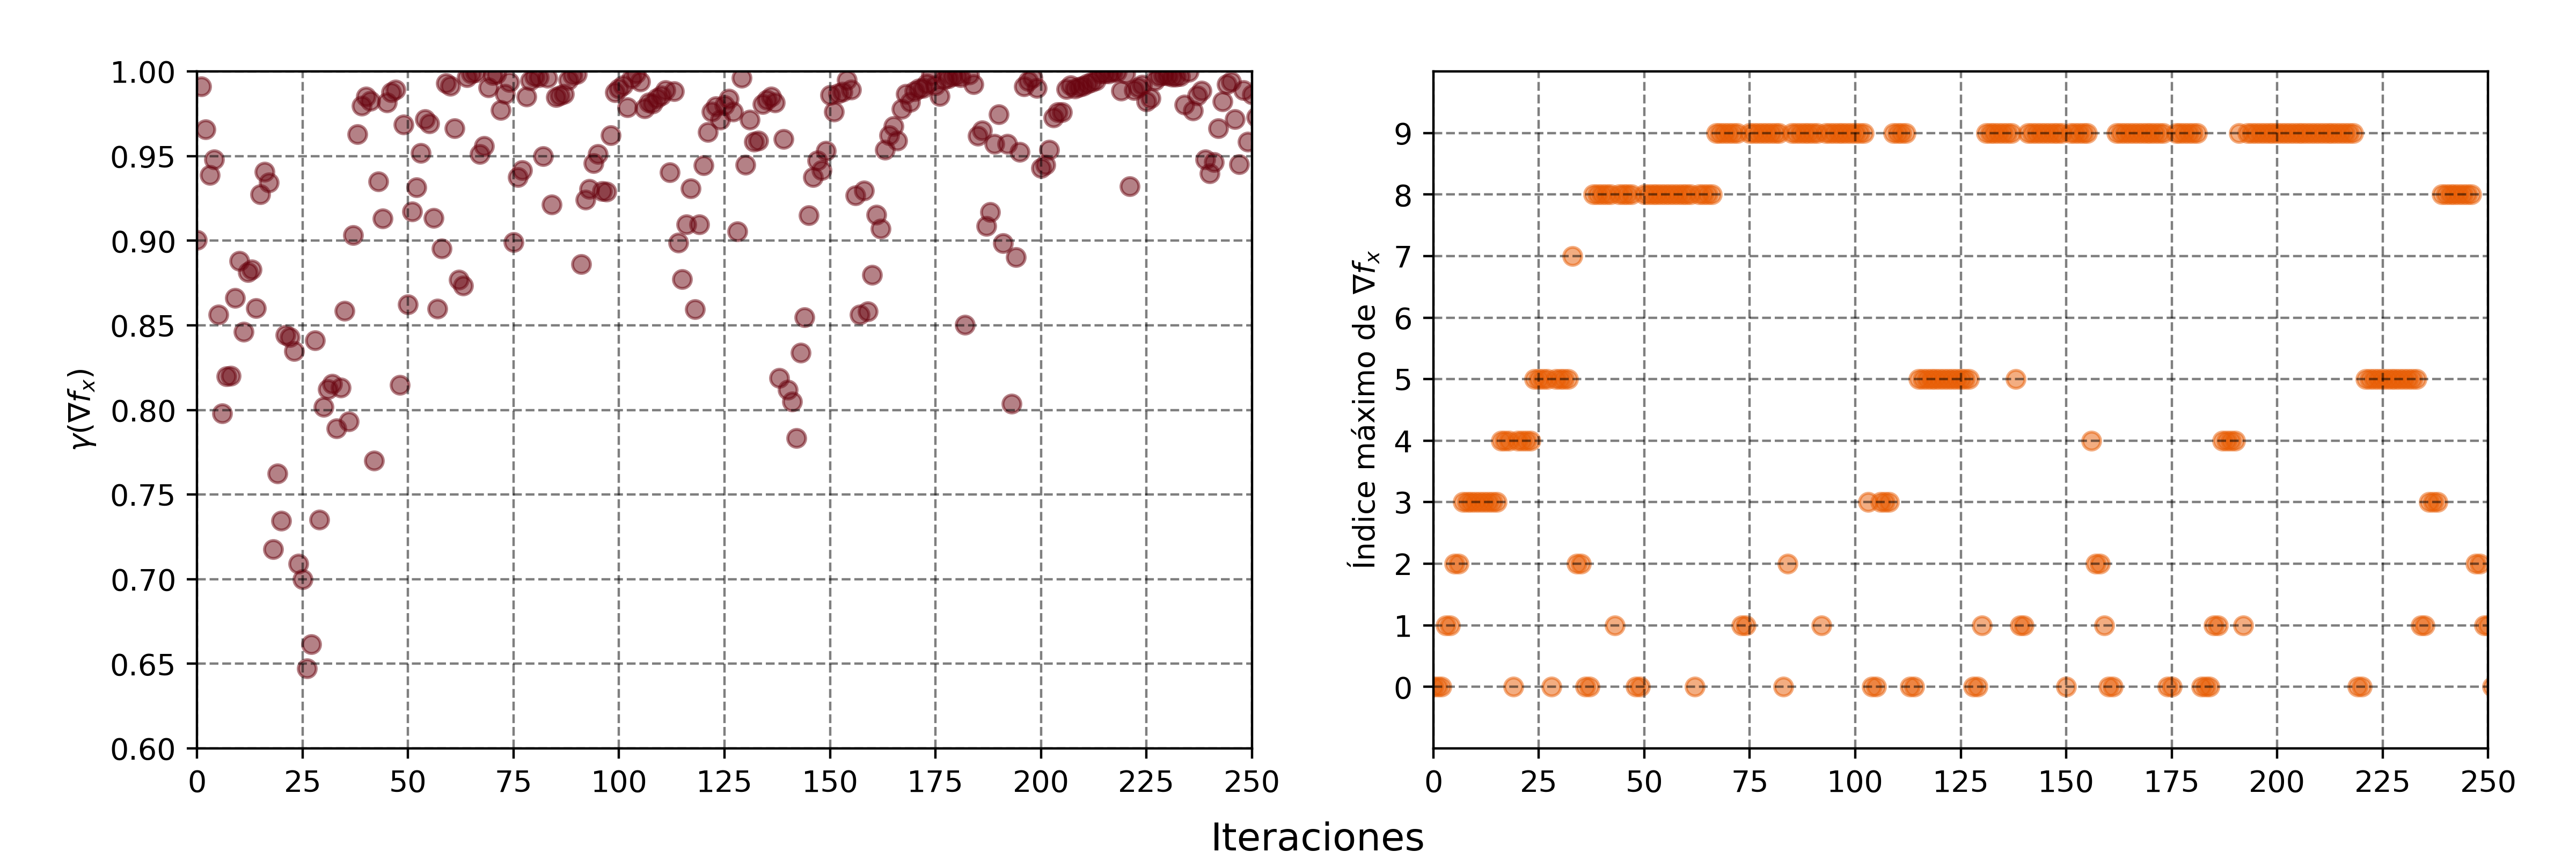
\includegraphics[width=1\textwidth]{Graphics/gamma/ANGR1.png}
            \caption{Método ANGR1}
        \end{subfigure}
        \begin{subfigure}{7cm}
            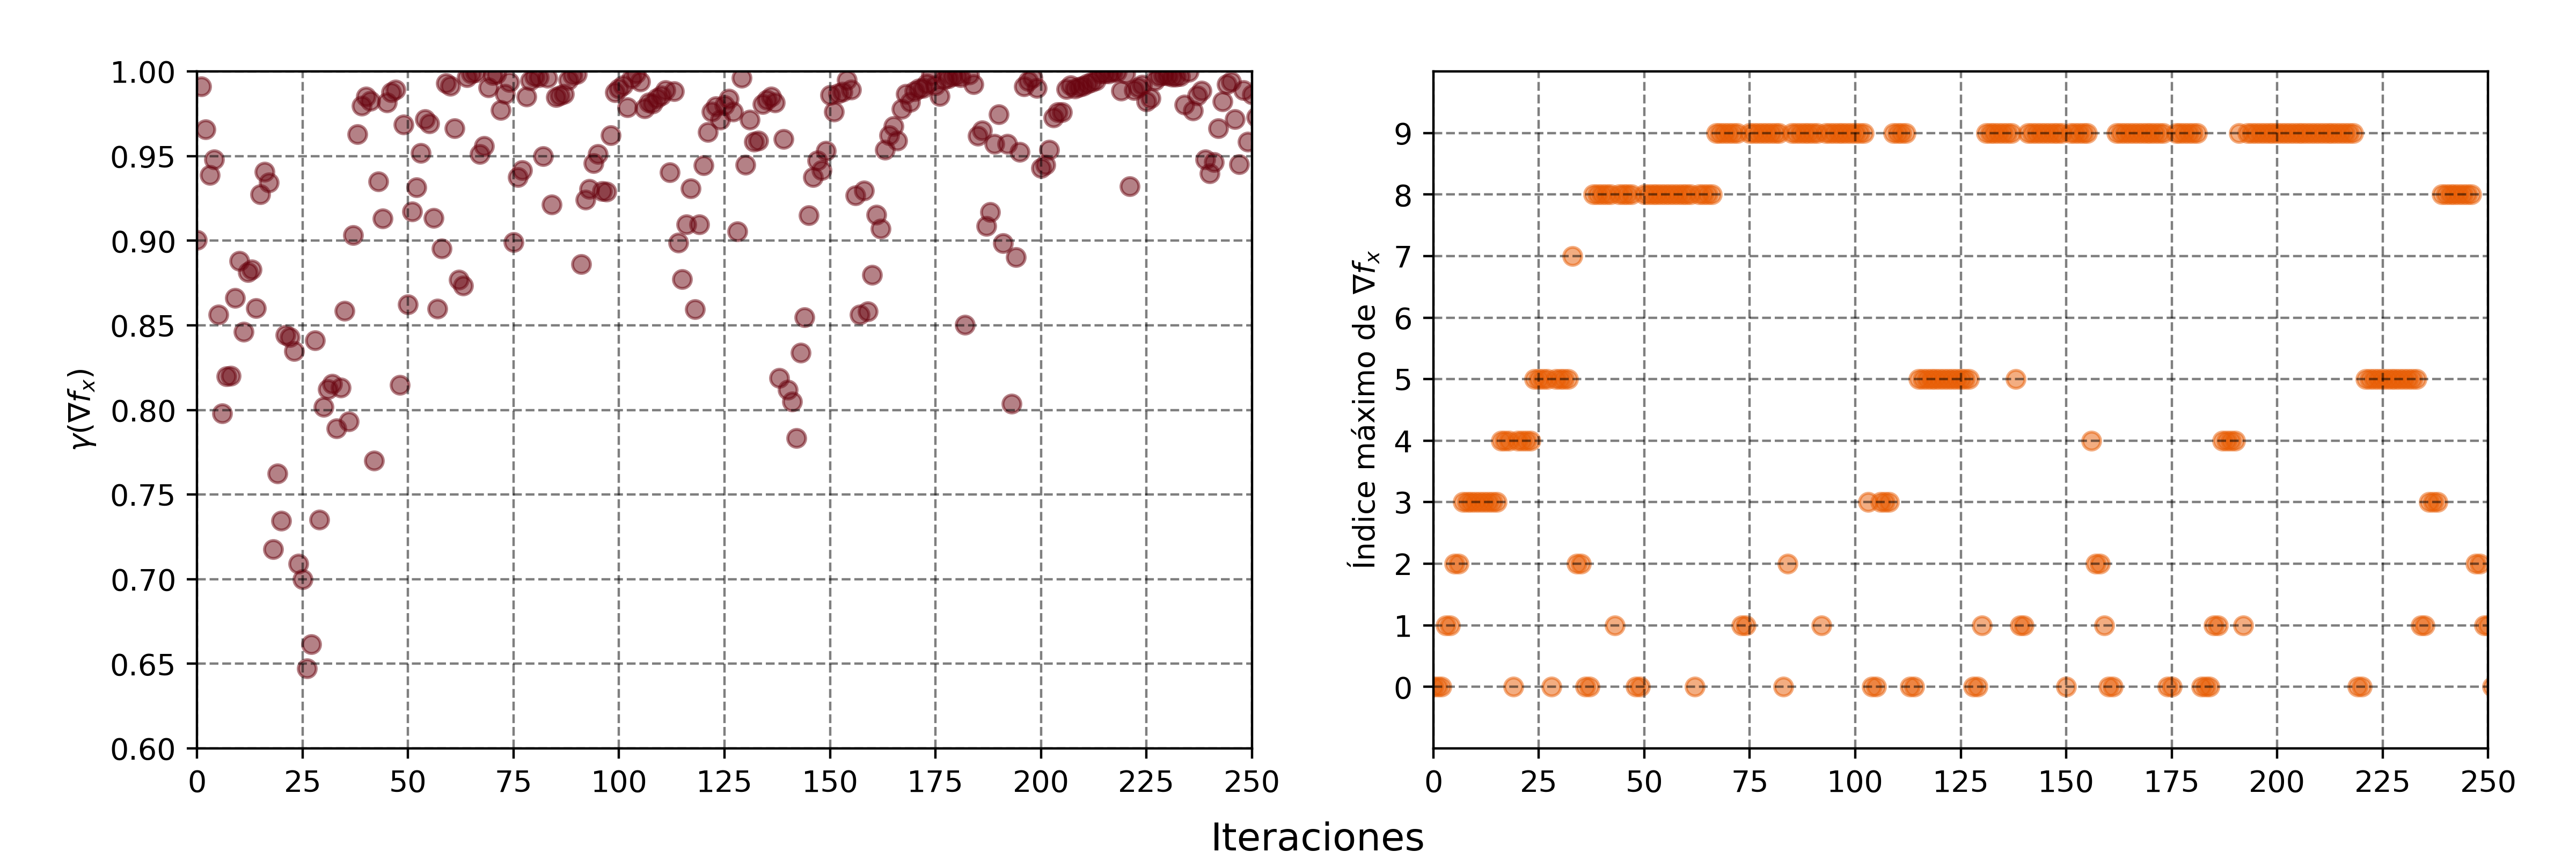
\includegraphics[width=1\textwidth]{Graphics/gamma/ANGR1.png}
            \caption{Método ANGR2.}
        \end{subfigure}
        \caption{\small Función $\gamma$ para diferentes métodos (izquierda) y la posición en el vector de la componente más grande (derecha).}
        \label{fig:gamma}
    \end{figure}
\end{frame}

\begin{frame}{\insertsectionhead}
    \framesubtitle{Porcentaje de contribución}
    \begin{table}[H]
    \centering
    \begin{tabular}{lrr}
        \hline
        \textbf{Método} & $\boldsymbol{\gamma(g_k)>0.8}$ & \textbf{Total} \\\hline
        SD              & 8057                           & 8104           \\
        BB              & 815                            & 851            \\
        ANGM            & 293                            & 316            \\
        ANGR1           & 240                            & 253            \\
        ANGR2           & 200                            & 245            \\ \hline
    \end{tabular}
    \caption{Número de iteraciones donde el valor de la función $\gamma$ tuvó un valor mayor a 0.8 para cada método de optimización.}
    \label{table:gamma_function}
\end{table}
\end{frame}

\begin{frame}{\insertsectionhead}
    \framesubtitle{Estabilidad de resultados}
    \begin{figure}[H]
        \centering
        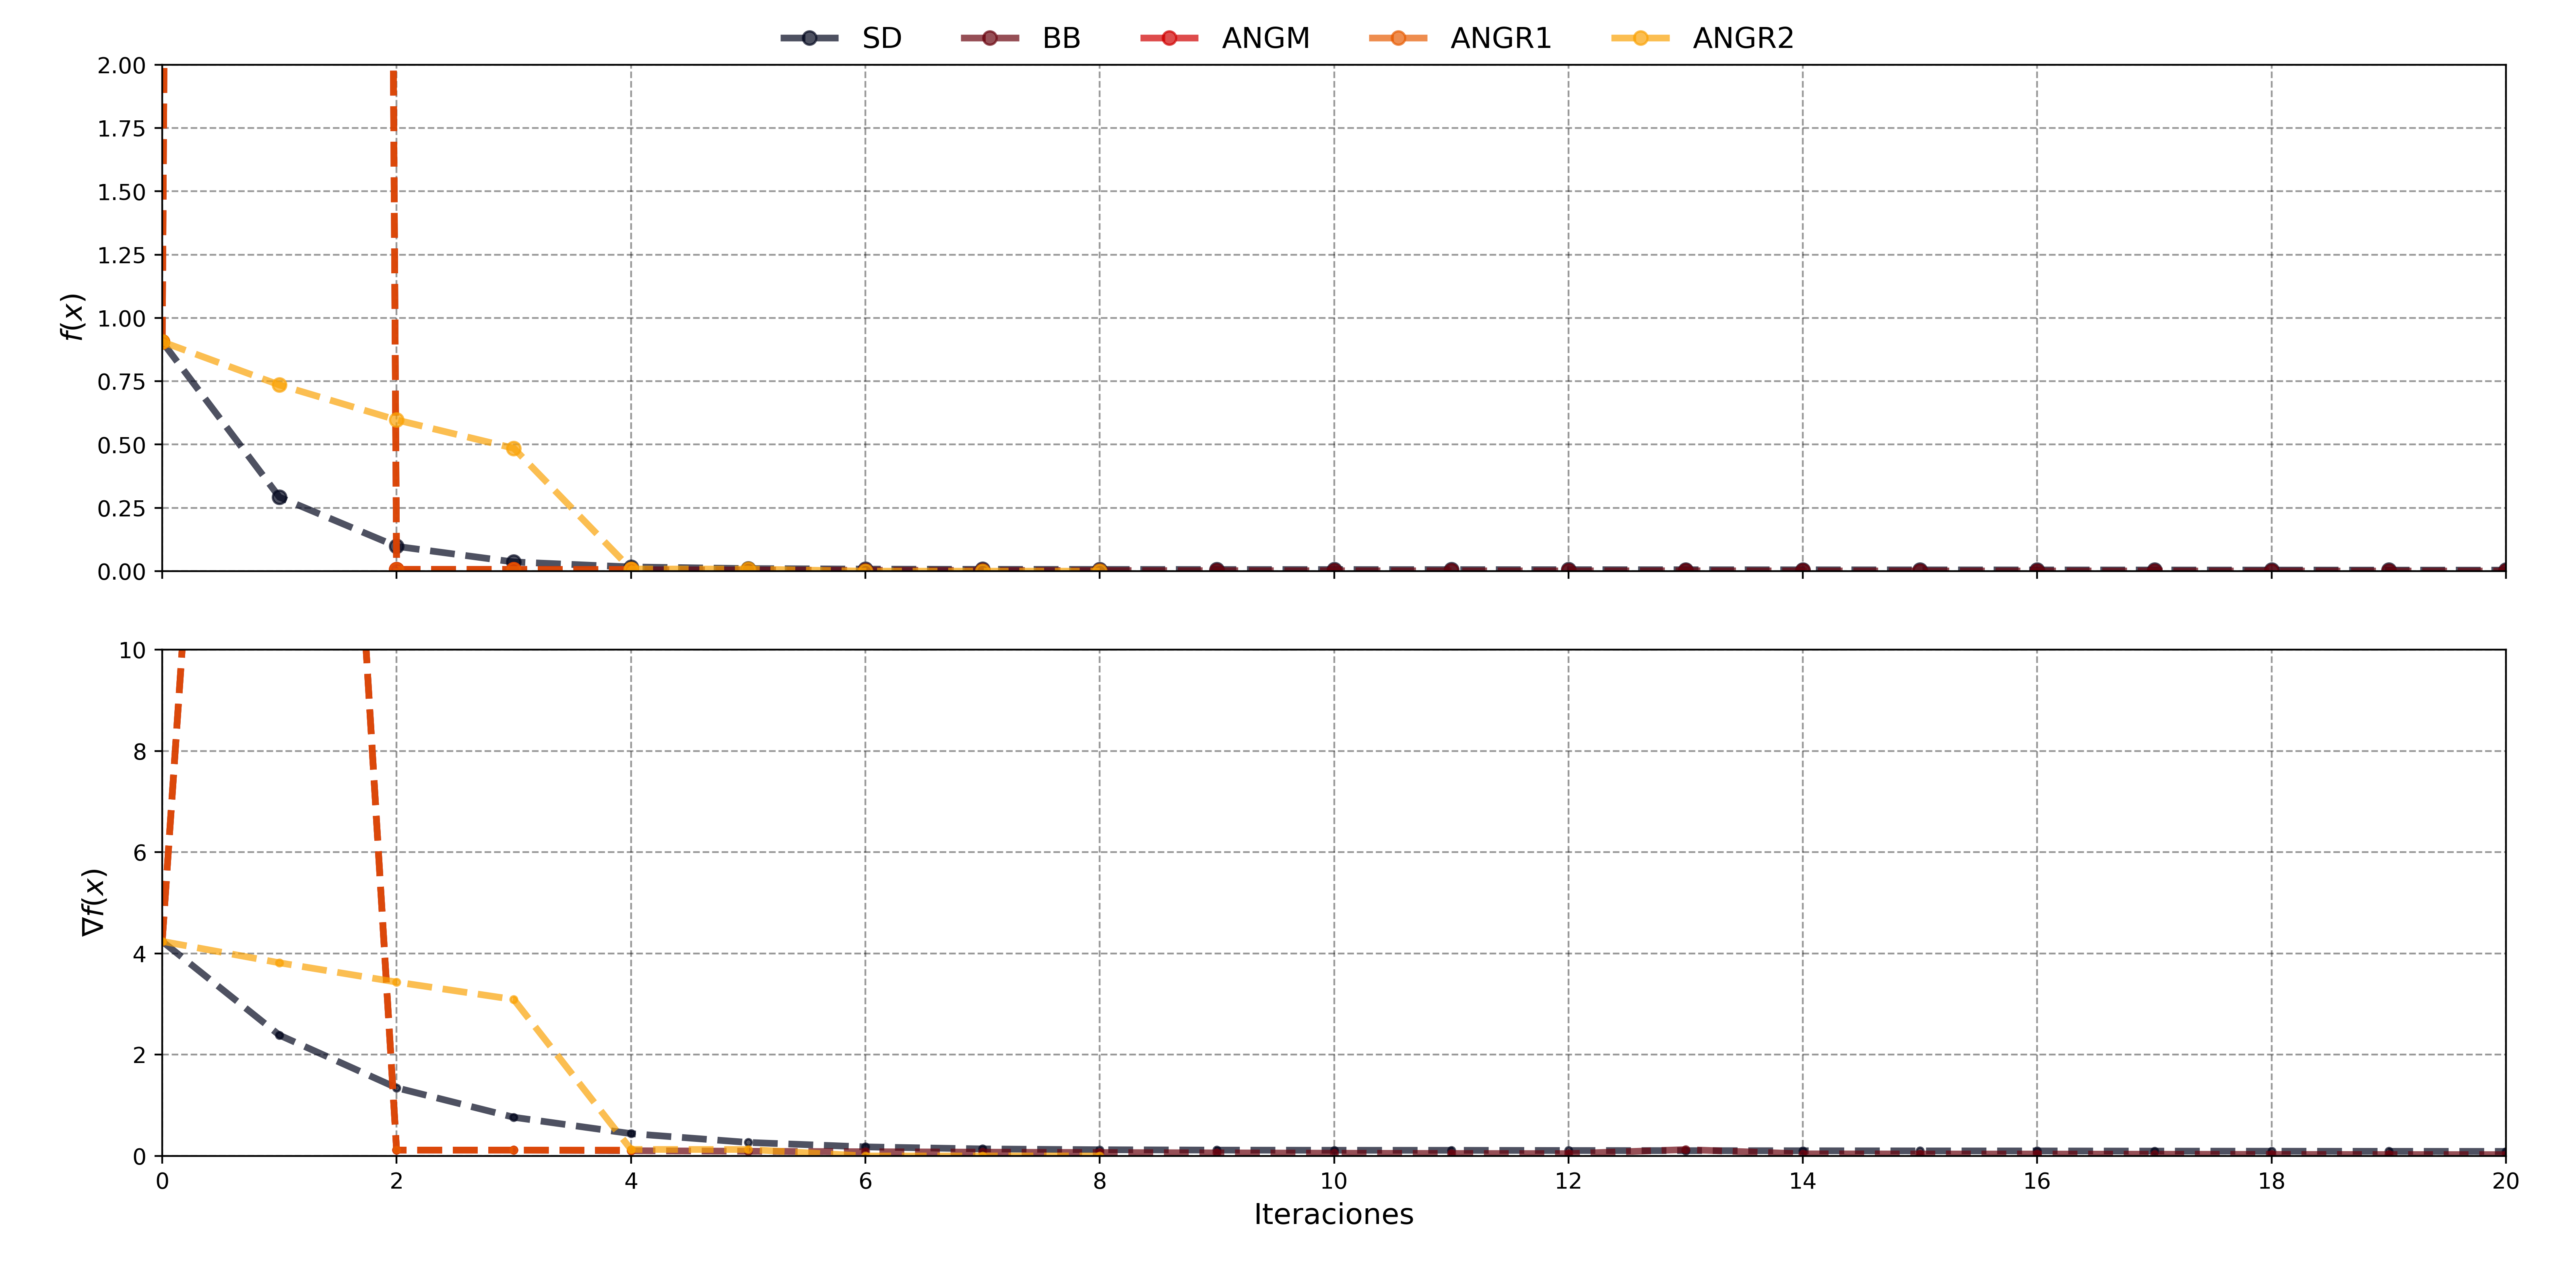
\includegraphics[width=10cm]{Graphics/function/quadratic.png}
        \caption{Valor de la función y norma del gradiente en cada iteración de la mejor ejecución de cada método de optimización de la función cuadrática con matriz diagonal.}
        \label{fig:quadracic_function}
    \end{figure}
\end{frame}

\begin{frame}{\insertsectionhead}
    \framesubtitle{Estabilidad de resultados}
    \begin{figure}[H]
        \centering
        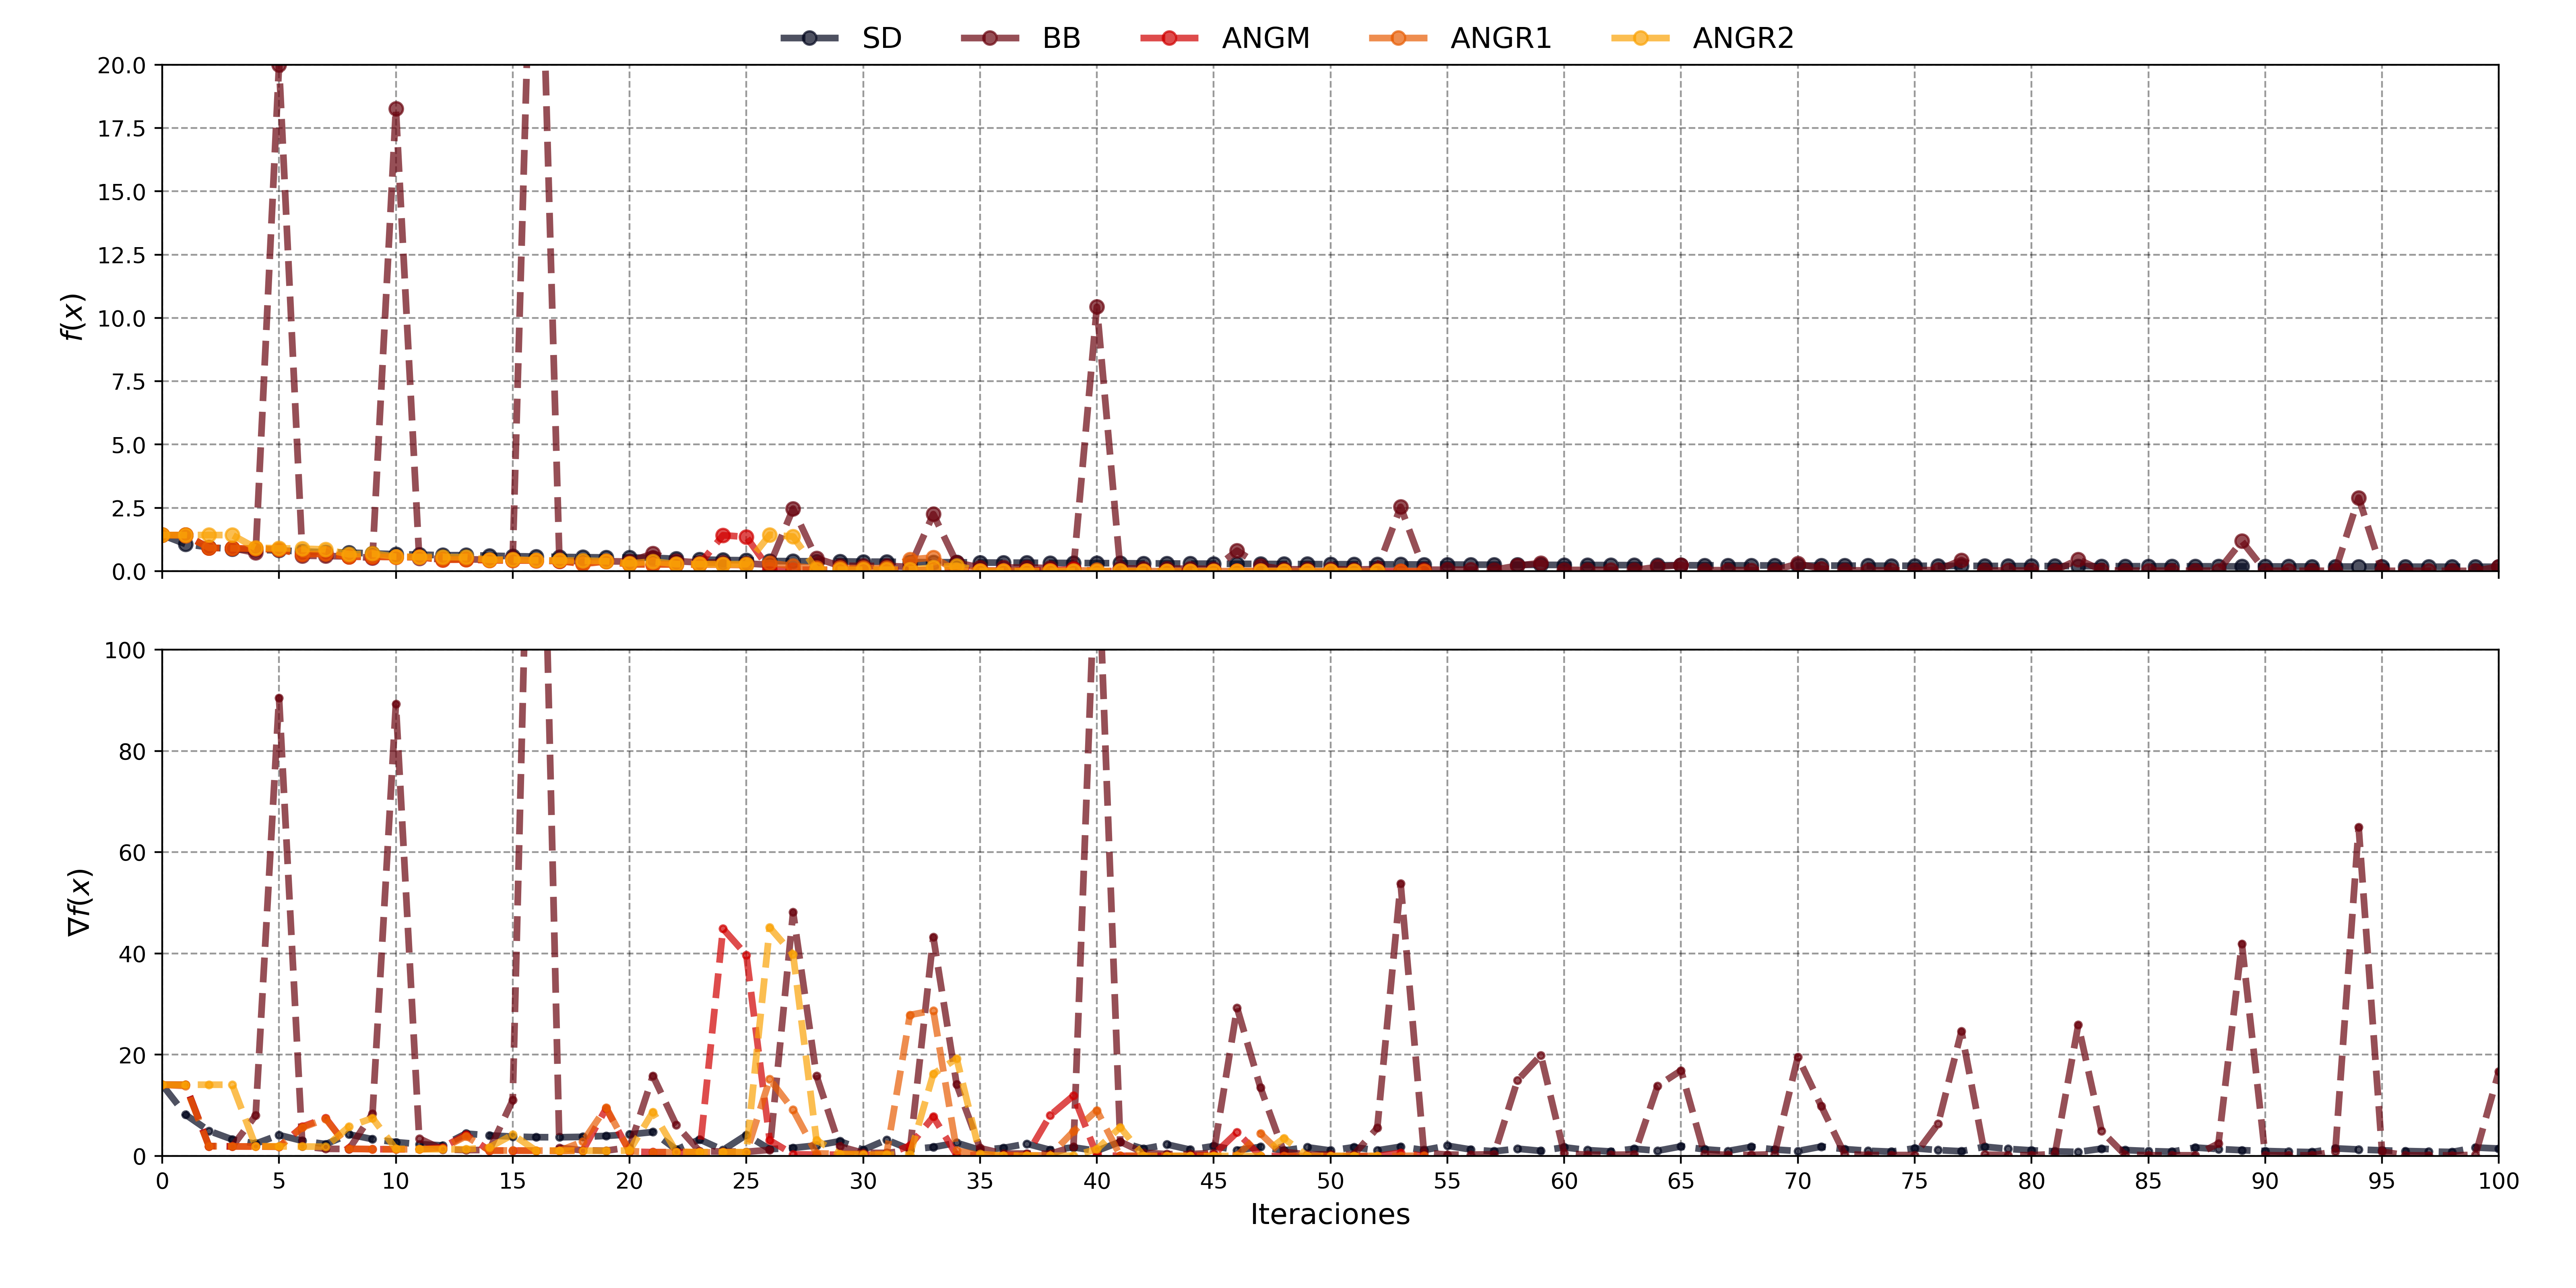
\includegraphics[width=10cm]{Graphics/function/rosembrock.png}
        \caption{Valor de la función y norma del gradiente en cada iteración de la mejor ejecución de cada método de optimización de la función de Rosembrock con matriz diagonal.}
        \label{fig:rosembrock_function}
    \end{figure}
\end{frame}

\begin{frame}
    \vspace{0.5cm}
    \begin{table}[H]
    \changefontsizes{10pt}
    \centering
    \begin{tabular}{llrrrrr}
        \hline                                                                                                           \\
        \textbf{Función} & \textbf{Valor} & \textbf{SD}  & \textbf{BB} & \textbf{ANGM} & \textbf{ANGR1} & \textbf{ANGR2} \\[0.1cm]\hline
        \\
                         & Función        & 0.000000     & 0.000000    & 0.000000      & 0.000000       & 0.000000       \\[0.25cm]
        Lambda           & Gradiente      & 0.000001     & 0.000001    & 0.000001      & 0.000001       & 0.000001       \\[0.25cm]
                         & Iteraciones    & 7764.810000  & 2770.340000 & 252.430000    & 289.490000     & 255.830000     \\[0.25cm]\hline
        \\
                         & Función        & 0.000000     & 0.000000    & 0.000000      & 0.000000       & 0.000000       \\[0.25cm]
        Cuadrática       & Gradiente      & 0.000001     & 0.000001    & 0.000000      & 0.000000       & 0.000000       \\[0.25cm]
                         & Iteraciones    & 713.000000   & 1531.230000 & 5.240000      & 7.360000       & 9.700000       \\[0.25cm]\hline
        \\
                         & Función        & 4.161332     & 42.245667   & 0.000000      & 0.000000       & 0.000000       \\[0.25cm]
        Rosembrock       & Gradiente      & 0.566027     & 45.446672   & 0.000000      & 0.000000       & 0.000000       \\[0.25cm]
                         & Iteraciones    & 10000.000000 & 1603.210000 & 68.840000     & 70.170000      & 67.150000      \\[0.25cm]\hline
        \\
                         & Función        & 0.000000     & 3.158103    & 5.070144      & 4.561704       & 8.428735       \\[0.25cm]
        Wood             & Gradiente      & 0.000004     & 0.000001    & 0.000000      & 0.000000       & 0.000000       \\[0.25cm]
                         & Iteraciones    & 9428.690000  & 1806.430000 & 360.360000    & 292.430000     & 199.210000     \\[0.25cm]\hline
    \end{tabular}
    \caption{Media de las 100 ejecucciones partiendo de puntos aleatorios.}
\end{table}
\end{frame}

\begin{frame}
    \vspace{0.5cm}
    \begin{table}[H]
    \small
    \centering
    \begin{tabular}{llrrrrr}
        \hline
        \textbf{Función} & \textbf{Valor} & \textbf{SD} & \textbf{BB} & \textbf{ANGM} & \textbf{ANGR1} & \textbf{ANGR2} \\[0.1cm]\hline
                         & Función        & 0.00        & 0.00        & 0.00          & 0.00           & 0.00           \\
        Lambda           & Gradiente      & 0.00        & 0.00        & 0.00          & 0.00           & 0.00           \\
                         & Iteraciones    & 612.38      & 209.34      & 32.55         & 28.34          & 25.04          \\\hline
                         & Función        & 0.00        & 0.00        & 0.00          & 0.00           & 0.00           \\
        Cuadrática       & Gradiente      & 0.00        & 0.00        & 0.00          & 0.00           & 0.00           \\
                         & Iteraciones    & 43.81       & 96.11       & 1.19          & 1.85           & 2.88           \\\hline
                         & Función        & 14.24       & 393.58      & 0.00          & 0.00           & 0.00           \\
        Rosembrock       & Gradiente      & 1.36        & 396.05      & 0.00          & 0.00           & 0.00           \\
                         & Iteraciones    & 0.00        & 1867.61     & 17.32         & 20.59          & 14.92          \\\hline
                         & Función        & 0.00        & 10.09       & 12.22         & 11.86          & 14.40          \\
        Wood             & Gradiente      & 0.00        & 0.00        & 0.00          & 0.00           & 0.00           \\
                         & Iteraciones    & 465.60      & 633.53      & 190.56        & 204.76         & 119.76         \\\hline
    \end{tabular}
    \caption{Desviaciones estandar de las 100 ejecucciones partiendo de puntos aleatorios.}
    \label{table:deviation}
\end{table}
\end{frame}